\section{Dependability e Security}
I veicoli a guida autonoma appartengono alla categoria dei sistemi critici. Un sistema critico è un sistema il cui malfunzionamento può provocare danni
considerati inacettabili. Questi includono danni a oggetti di valore, danni ambientali e nei casi piu gravi, il ferimento o addirittura la morte delle persone.
Per garantire che un tale sistema operi nel modo più sicuro possibile è necessario analizzare tutti i fattori che possono portare a  un fallimento irreversibile.

\subsection{Dependability}
La dependability è la capacità di un sistema di fornire un servizio sul quale è possibile fare affidamento in modo giustificato.
Essa viene suddivisa in 3 categorie:
\begin{itemize}
    \item Attributi
    \item Minacce
    \item Mezzi di Raggiungimento
\end{itemize}
\begin{figure}[h]
    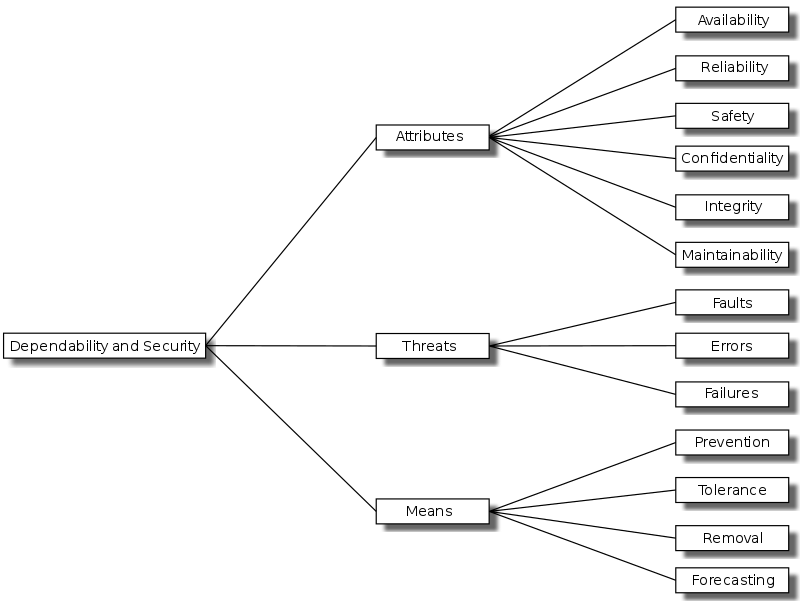
\includegraphics[width = \linewidth]{dep.png}
    \caption{tassonomia  della dependability\cite{dep}}
    \label{fig:dep}
\end{figure}
\subsubsection{Attributi}
